\documentclass[
  bibliography=totoc,     % Literatur im Inhaltsverzeichnis
  captions=tableheading,  % Tabellenüberschriften
  titlepage=firstiscover, % Titelseite ist Deckblatt
]{scrartcl}

% Paket float verbessern
\usepackage{scrhack}

% Warnung, falls nochmal kompiliert werden muss
\usepackage[aux]{rerunfilecheck}

% unverzichtbare Mathe-Befehle
\usepackage{amsmath}
% viele Mathe-Symbole
\usepackage{amssymb}
% Erweiterungen für amsmath
\usepackage{mathtools}

% Fonteinstellungen
\usepackage{fontspec}
% Latin Modern Fonts werden automatisch geladen
% Alternativ:
%\setromanfont{Libertinus Serif}
%\setsansfont{Libertinus Sans}
%\setmonofont{Libertinus Mono}
\recalctypearea % Wenn man andere Schriftarten gesetzt hat,
% sollte man das Seiten-Layout neu berechnen lassen

% deutsche Spracheinstellungen
\usepackage{polyglossia}
\setmainlanguage{german}


\usepackage[
  math-style=ISO,    % ┐
  bold-style=ISO,    % │
  sans-style=italic, % │ ISO-Standard folgen
  nabla=upright,     % │
  partial=upright,   % ┘
  warnings-off={           % ┐
    mathtools-colon,       % │ unnötige Warnungen ausschalten
    mathtools-overbracket, % │
},                       % ┘
]{unicode-math}

% traditionelle Fonts für Mathematik
\setmathfont{Latin Modern Math}
% Alternativ:
%\setmathfont{Libertinus Math}

\setmathfont{XITS Math}[range={scr, bfscr}]
\setmathfont{XITS Math}[range={cal, bfcal}, StylisticSet=1]

% Zahlen und Einheiten
\usepackage[
locale=DE,                   % deutsche Einstellungen
separate-uncertainty=true,   % immer Fehler mit \pm
per-mode=symbol-or-fraction, % / in inline math, fraction in display math
]{siunitx}

% chemische Formeln
\usepackage[
version=4,
math-greek=default, % ┐ mit unicode-math zusammenarbeiten
text-greek=default, % ┘
]{mhchem}

% richtige Anführungszeichen
\usepackage[autostyle]{csquotes}

% schöne Brüche im Text
\usepackage{xfrac}

% Standardplatzierung für Floats einstellen
\usepackage{float}
\floatplacement{figure}{htbp}
\floatplacement{table}{htbp}

% Floats innerhalb einer Section halten
\usepackage[
section, % Floats innerhalb der Section halten
below,   % unterhalb der Section aber auf der selben Seite ist ok
]{placeins}

% Seite drehen für breite Tabellen: landscape Umgebung
\usepackage{pdflscape}

% Captions schöner machen.
\usepackage[
  labelfont=bf,        % Tabelle x: Abbildung y: ist jetzt fett
  font=small,          % Schrift etwas kleiner als Dokument
  width=0.9\textwidth, % maximale Breite einer Caption schmaler
]{caption}
% subfigure, subtable, subref
\usepackage{subcaption}

% Grafiken können eingebunden werden
\usepackage{graphicx}
% größere Variation von Dateinamen möglich
\usepackage{grffile}

% schöne Tabellen
\usepackage{booktabs}

% Verbesserungen am Schriftbild
\usepackage{microtype}

% Literaturverzeichnis
\usepackage[style=alphabetic,]{biblatex}
% Quellendatenbank
\addbibresource{lit.bib}

% Hyperlinks im Dokument
\usepackage[
  unicode,        % Unicode in PDF-Attributen erlauben
  pdfusetitle,    % Titel, Autoren und Datum als PDF-Attribute
  pdfcreator={},  % ┐ PDF-Attribute säubern
  pdfproducer={}, % ┘
]{hyperref}
% erweiterte Bookmarks im PDF
\usepackage{bookmark}

% Trennung von Wörtern mit Strichen
\usepackage[shortcuts]{extdash}

\title{V206: Die Wärmepumpe}
\author{
  Simon Schulte
  \texorpdfstring{
    \\
    \href{mailto:simon.schulte@udo.edu}{simon.schulte@udo.edu}
  }{}
  \texorpdfstring{\and}{, }
  Tim Sedlaczek
  \texorpdfstring{
    \\
    \href{mailto:tim.sedlaczek@udo.edu}{tim.sedlaczek@udo.edu}
  }{}
}
\publishers{TU Dortmund – Fakultät Physik}

\date{Durchführung: 02.02.2017\\
      Abgabe: 09.02.2017}


\begin{document}

\maketitle
\thispagestyle{empty}
\tableofcontents
\newpage
\section{Zielsetzung}
\label{sec:zielsetzung}
Ziel des Versuchs ist die Untersuchung einer mechanischen Wärmepumpe.
\section{Theorie}
\label{sec:theorie}
Wärmepumpen werden genutzt, um Objekte moglichst effizient zu erwärmen.
Es ist mit Wärmepumpen möglich kalten Objekten Wärme zu entziehen und diese
entzogene Wärme widerum warmen Objekten hinzuzufügen. In der Natur ist zu
beobachten, dass Wärmeenergie immer danach strebt von einem wärmeren in ein
kälteres Raumgebiet zu gelangen. Um aber Wärmeenergie von einem kälteren Gebiet
in ein wärmeres zu bringen muss zusätztlich Energie zugeführt werden.
In diesem Versuch wird das durch mechanische Arbeit gewährleistet. Diese wird
von einer Wärmepumpe erbracht. \\
\\
Wird von einem Wärmereservoir die Wärmeenergie
$Q_2$ entnommen und einem anderen Reservoir zugefügt, so geht nach dem ersten
Hauptsatz der Thermodynamik auch zusätzlich die dazu benötigte Arbeit $A$ mit
in die Energiebilanz ein. Daraus folgt die an das wärmere Reservoir abgegebene
Wärmemenge $Q_1$ mit
\begin{equation}
    Q_1=Q_2+A.
    \label{eqn:wärmebilanz}
\end{equation}
Eine charakteristische Größe einer Wärmepumpe ist die Güteziffer $ν$, welche der
Quotient aus transportierter Wärmemenge $Q_1$ und dazu aufgewendeter Arbeit $A$
ist.
\begin{equation}
    \nu=\frac{Q_1}{A}
    \label{eqn:güteziffer}
\end{equation}
Für den Fall einer vollständig reversiblen Wärmeübertragung folgt aus dem
zweiten Hauptsatz der Thermodynamik mit den Temperaturen $T_1$ und $T_2$:
\begin{equation}
    \frac{Q_1}{T_1}=\frac{Q_2}{T_2}
    \label{eqn:idealisierende_annahme}
\end{equation}
Für diesen Idealfall ergibt sich aus den
Gleichungen~\eqref{eqn:wärmebilanz}~--~\eqref{eqn:idealisierende_annahme} für die
Güteziffer der Zusammenhang
\begin{equation}
    \nu_{\mathup{ideal}}=\frac{T_1}{T_1-T_2}.
	\label{eqn:guete_ideal}
\end{equation}
Eine ideale Maschine ist jedoch nicht realisierbar, da beim
Übertragungsprozess immer ein Teil der Energie das System irreversibel verlässt.
Damit gilt
\begin{align}
  \frac{Q_1}{T_1}>\frac{Q_2}{T_2}\qquad\text{und somit}\qquad ν_{\mathup{real}}<\frac{T_1}{T_1-T_2}.
    \label{eqn:ungleichungen}
\end{align}
Um die reale Güteziffer der Wärmepumpe zu bestimmen werden die gemessenen
Messwerte genutzt und es gilt
\begin{equation}
    \nu_{\mathup{real}}=\frac{\mathup{Δ}Q_1}{\mathup{Δ}t\,N}=(m_1 c_{\mathup{w}}+m_{\mathup{k}}c_{\mathup{k}})\frac{\mathup{Δ}T_1}{\mathup{Δ}t\,N}.
	\label{eqn:guete_real}
\end{equation}
$N$ bezeichnet die zeitlich gemittelte Leistung des verwendeten
Kompressors. $m_1 c_{\mathup{w}}$ und $m_{\mathup{k}}c_{\mathup{k}}$ bezeichnen
die Wärmekapazität des Wasser bzw. der Kupferschlange und
$\sfrac{\mathup{Δ}T_1}{\mathup{Δ}t}$ bezeichnet den zeitlichen Temperaturverlauf
im ersten Reservoir. \\
\\
Eine weitere charakteristische Größe der Wärmepumpe ist ihr Massendurchsatz
$\sfrac{\mathup{Δ}m}{\mathup{Δ}t}$, welcher aus einer Betrachtung der
Wärmeänderung im kalten Reservoir folgt:
\begin{equation}
    \frac{\mathup{Δ}Q_2}{\mathup{Δ}t}=(m_2 c_{\mathup{w}}+m_{\mathup{k}}c_{\mathup{k}})\frac{\mathup{Δ}T_2}{\mathup{Δ}t}.
    \label{eqn:massendurchsatz}
\end{equation}
Der Zusammenhang zum Massendurchsatz erfolgt unter Zuhilfenahme der
Verdampfungswärme des Transportmediums. Ist diese bekannt, ermittelt sich der
Massendurchsatz zu:
\begin{equation}
    \frac{\mathup{Δ}m}{\mathup{Δ}t}=\frac{\mathup{Δ}Q_2}{L \cdot \mathup{Δ}t}.
	\label{eqn:massen_umsatz}
\end{equation}
\\
Die dritte interessante charakteristische Größe ist die mechanische Leistung
$N_{\mathup{mech}}$ des Kompressors. Diese ergibt sich bei angenommener
adiabatischer Kompression aus der Poissonschen Gleichung zu:
\begin{equation}
    N_{\mathup{mech}}=\frac{1}{κ-1}\left(p_{\mathup{b}}\sqrt[κ]{\frac{p_{\mathup{a}}}{p_{\mathup{b}}}}-p_{\mathup{a}}\right)\frac{1}{ρ}\frac{\mathup{Δ}m}{\mathup{Δ}t}.
	\label{eqn:Leistung}
\end{equation}
$\kappa$ bezeichnet hierbei das Verhältnis der Molwärmen $C_{\mathup{p}}$ und
$C_{\mathup{V}}$, $p_{\mathup{a}}$ und $p_{\mathup{b}}$ die aufgenommenen Drücke
und $\rho$ die Dichte des zirkulierenden Mediums in der Gasphase. Diese errechnet
sich aufgrund der adiabatischen Kompression mit Hilfe der idealen Gasgleichung
aus der Dichte $\rho_0$ unter Normalbedingungen. Dabei wird
\begin{equation}
    \frac{p_{\SI{0}{\celsius}}}{ρ_0T_0}=\frac{p_{\mathup{a}}}{ρ\;T_{\mathup{2}}}
\end{equation}
umgeformt zu:
\begin{equation}
    ρ=\frac{p_{\mathup{a}}T_0}{p_{\SI{0}{\celsius}}T_{\mathup{2}}}ρ_0.
	\label{eqn:dichte}
\end{equation}
\section{Durchführung}
\label{sec:durchführung}
\begin{figure}[htb]
  \centering
  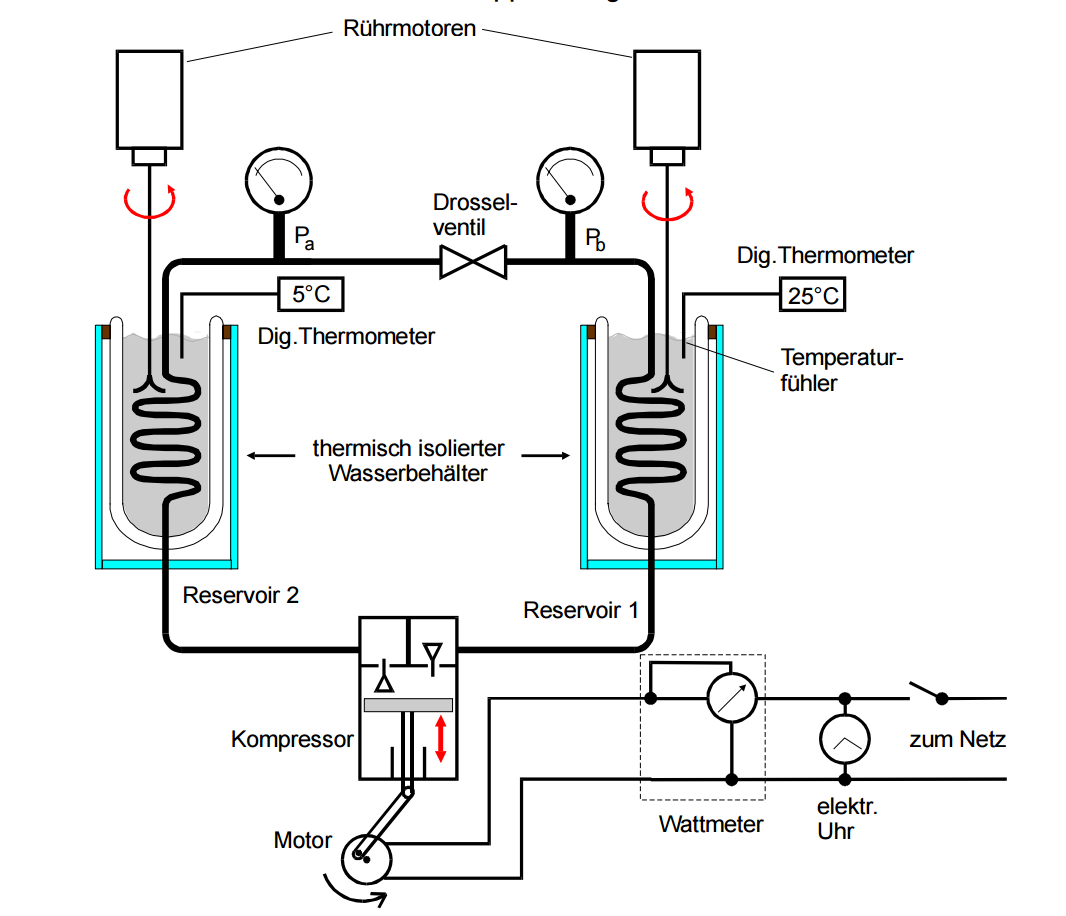
\includegraphics[width=0.99\textwidth]{V2062.png}
  \caption{Der Versuchsaufbau der Messapparatur \cite{anleitung}.}
  \label{fig:V2062}
\end{figure}
In Abbildung \ref{fig:V2062} zu sehen ist der schematische Aufbau der
verwendeten Wärmepumpe. Als Transportmedium zirkuliert angetrieben von einem
Kompressor das Gas Dichloridfluormethan $(Cl_2F_2C)$. Durch das Drosselventil
wird ein Druckunterschied innerhalb der Apparatur erzeugt, sodass in der
Kupferspirale vom zweiten Reservoir das Medium verdampft und dem Wasser dabei die
erforderliche Verdampfungswärme $Q_2$ entzieht. Das Medium wird daraufhin
adiabatisch komprimiert und in die Kupferspirale von Reservoir 1 geleitet.
Dort wird es infolge des höheren Drucks kondensiert und die aufgenommene Wärmemenge
$Q_2+A$ wird abgegeben. Neben zwei Thermometern, die Temperatur messen und 2
Manometern, die den Druck auf beiden Seiten des Kompressors bzw. des
Drosselventils angeben, ist an dem Kompressor noch zusätzlich ein Wattmeter
angeschlossen. Dieses zeigt die elektrische Leistung als Maß für die verrichtete
mechanische Arbeit an. Um eine gleichmäßige Wärmeverteilung innerhalb der
Wasserreservoirs zu gewährleisten werden zwei Rührmotoren verwendet.

\subsection{Versuchsablauf}
\label{sub:versuchsablauf}
Die beiden Reservoirs werden beide mit je 3 Liter Leitungswasser
gleicher Temperatur befüllt. Nachdem man die Wärmepumpe eingeschaltet hat, werden
die Parameter $p_{\mathup{a}}$, $p_{\mathup{b}}$, $T_1$, $T_2$ und $N$ pro Minute
aufgenommen. Der Versuch endet, wenn das erste Reservoir eine Temperatur von
$\SI{50}{\celsius}$ erreicht.
\clearpage
\section{Auswertung}
\label{sec:auswertung}
\subsection{Fehlerrechnung}
Die Fehler werden im Folgenden mit Python berechnet. Dabei wird das Paket "uncertainties"
verwendet. Dieses berechnet die Fehler nach der Gaußschen Fehlerfortpflanzung.
\begin{equation}
    \mathup{\Delta}f(x_1,x_2,...,x_n)=\sqrt{\left(\frac{\mathup{d}f}{\mathup{d}x_1}\mathup{\Delta}x_1\right)^2+\left(\frac{\mathup{d}f}{\mathup{d}x_2}\mathup{\Delta}x_2\right)^2+ \dotsb +\left(\frac{\mathup{d}f}{\mathup{d}x_n}\mathup{\Delta}x_n\right)^2}.
    \label{eqn:formelgauß}
\end{equation}
\subsection{Bestimmung der Güteziffer}
\begin{table}
  \centering
  \caption{Gemessene Temperaturen und Leistung zur jeweiligen Zeit.}
  \label{tab:messwerte1}
  \sisetup{table-format=3.2}
  \begin{tabular}{S S S[table-format=3.1] S[table-format=4.0]}
    \toprule
    {$T_1 \,/\, \si{\kelvin}$} & {$T_2 \,/\, \si{\kelvin}$} & {$N \,/\, \si{\watt}$} & {$t \,/\, \si{\second}$}\\
    \midrule
    294.35 & 294.25 & 0.0 & 0\\
    295.35 & 294.25 & 165.0 & 60\\
    296.15 & 294.15 & 175.0 & 120\\
    297.45 & 293.05 & 185.0 & 180\\
    299.05 & 291.65 & 192.5 & 240\\
    300.95 & 289.95 & 200.0 & 300\\
    302.95 & 288.05 & 202.5 & 360\\
    304.95 & 286.15 & 205.0 & 420\\
    306.85 & 284.35 & 207.5 & 480\\
    308.75 & 282.45 & 207.5 & 540\\
    310.25 & 280.85 & 210.0 & 600\\
    312.35 & 279.15 & 210.0 & 660\\
    314.15 & 277.55 & 212.5 & 720\\
    315.75 & 276.05 & 212.5 & 780\\
    317.35 & 274.75 & 215.0 & 840\\
    318.95 & 273.85 & 212.5 & 900\\
    320.35 & 273.15 & 212.5 & 960\\
    321.75 & 272.65 & 210.0 & 1020\\
    323.15 & 272.15 & 207.5 & 1080\\
    \bottomrule
  \end{tabular}
\end{table}
Zu Beginn werden die gemessenen Temperaturen aus Tabelle \ref{tab:messwerte1}
in Abhängigkeit von der Zeit aufgetragen und durch geeignete Funktionen genähert.
Die Näherungen werden dabei mit Python durchgeführt.
Für die Temperaturen $T_1$ des warmen Behälters wird ein Polynom der Gestalt
\begin{equation}
  T_1 \left( t \right) = \mathup{A} t^3 + \mathup{B} t^2 + \mathup{C} t + \mathup{D}
\end{equation}
verwendet, während für die Temperatur am kalten Behälter ($T_2$) eine Funktion
der Form
\begin{equation}
  T_2 \left( t \right) = \frac{\mathup{E} t^2}{1 + \mathup{F} t^2} + \mathup{G}
\end{equation}
verwendet wird.\\
\\
Damit ergeben sich die Parameter der Funktionen zu:
\begin{align}
  \mathup{A} &= \SI{-1.8(2)e-8}{\kelvin\cdot\second\tothe{-3}} &  &\mathup{B} = \SI{-2.9(3)e-5}{\kelvin\cdot\second\tothe{-2}}\\
  \mathup{C} &= \SI{1.6(2)e-2}{\kelvin\cdot\second\tothe{-1}} &  &\mathup{D} = \SI{294.1(2)}{\kelvin}\\
  \mathup{E} &= \SI{-6.8(3)e-5}{\kelvin\cdot\second\tothe{-2}} &  &\mathup{F} = \SI{2.1(1)e-6}{\second\tothe{-2}}\\
  \mathup{G} &= \SI{294.9(2)}{\kelvin} &  &
\end{align}\\
Der entsprechende Graph ist in Abbildung \ref{fig:plot1} zu sehen.
\begin{figure}[htb]
  \centering
  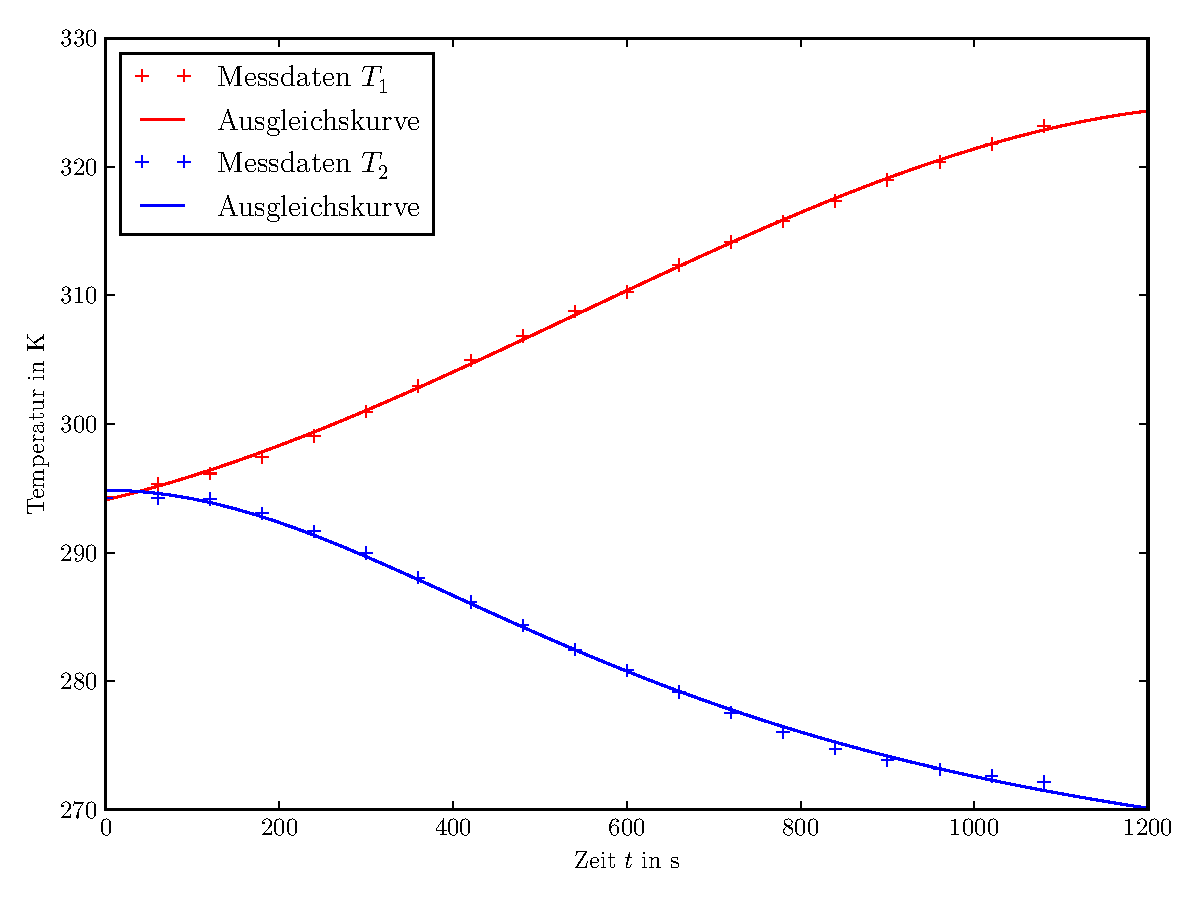
\includegraphics[width=\textwidth]{Plot.pdf}
  \caption{Temperaturen des Wassers in Abhängigkeit von der verstrichenen Zeit.}
  \label{fig:plot1}
\end{figure}\\
Nun werden die Ableitungen der Funktionen für je vier verschiedene Temperaturen
bestimmt.\\
Die Ableitungen haben dabei die Formen
\begin{equation}
  \frac{\symup{d} T_1 \left( t \right)}{\symup{d} t} = 3 A t^2+ 2 B t + C
\end{equation}
und
\begin{equation}
  \frac{\symup{d} T_2 \left( t \right)}{\symup{d} t} = \frac{2 D t}{\left(1 + E t^2 \right)^2}.
\end{equation}
Für die Zeiten $t = \SI{120}{\second}$, $t = \SI{420}{\second}$, $t = \SI{720}{\second}$
und $t = \SI{960}{\second}$ werden diese konkret berechnet. Die Ergebnisse stehen
in Tabelle \ref{tab:ergebnisse1}.
\begin{table}
  \centering
  \caption{Werte der Ableitungen von $T_1$ und $T_2$.}
  \label{tab:ergebnisse1}
  \sisetup{table-format=3.2}
  \begin{tabular}{S S S[table-format=3.0]}
    \toprule
    {$\frac{\symup{d} T_1 \left( t \right)}{\symup{d} t} \,/\, \si{\kelvin\per\second}$} & {$\frac{\symup{d} T_2 \left( t \right)}{\symup{d} t} \,/\, \si{\kelvin\per\second}$} & {$t \,/\, \si{\second}$}\\
    \midrule
    \num{2.2(2)e-2} & \num{-1.5(1)e-2} & 120\\
    \num{3.1(3)e-2} & \num{-3.1(2)e-2} & 420\\
    \num{3.0(6)e-2} & \num{-2.3(2)e-2} & 720\\
    \num{2.2(9)e-2} & \num{-1.6(1)e-2} & 960\\
    \bottomrule
  \end{tabular}
\end{table}\\
Aufgrund der Füllmenge von $\SI{3}{\liter}$ ergibt sich
\begin{equation}
  m_1 = \SI{3}{\kilo\gram}.
\end{equation}
Die Wärmekapazität von Wasser wird mit
\begin{equation}
  c_\mathup{w} = \SI{4180}{\joule\per\kilo\per\gram\per\kelvin}
\end{equation}
angenommen \cite{dulong}.
Außerdem wurde die Wärmekapazität der Apparatur zu
\begin{equation}
  m_\mathup{k}c_\mathup{k} = \SI{660}{\joule\per\kelvin}
\end{equation}
angegeben.
Mit diesen Werten und denen aus den Tabellen \ref{tab:messwerte1} und \ref{tab:ergebnisse1}
ergeben sich nach Formel \eqref{eqn:guete_real} dann folgende Werte für die reale Güte:
\begin{align}
  \nu_{\SI{296.15}{\kelvin}} &= \num{1.7(1)} & &\nu_{\SI{304.95}{\kelvin}} = \num{2.0(2)}\\
  \nu_{\SI{314.15}{\kelvin}} &= \num{1.9(4)} & &\nu_{\SI{320.35}{\kelvin}} = \num{1.4(6)}
\end{align}
Die Fehler wurden mit Hilfe von Python bestimmt.
Dabei lautet die Ableitung, die in Formel \eqref{eqn:formelgauß} verwendet wird:
\begin{equation}
  \frac{\partial \nu_\mathup{ideal}}{\partial \frac{\symup{d} T_1 \left( t \right)}{\symup{d} t}} = \frac{(m_1c_\symup{w}+m_\symup{k}c_\symup{k})}{N}.
\end{equation}
Die Werte der idealen Güte berechnen sich nach Formel \eqref{eqn:guete_ideal} zu
\begin{align}
  \nu_{\text{id}\,\SI{296.15}{\kelvin}} &= \num{148.1} & &\nu_{\text{id}\,\SI{304.95}{\kelvin}} = \num{16.2}\\
  \nu_{\text{id}\,\SI{314.15}{\kelvin}} &= \num{8.6} & &\nu_{\text{id}\,\SI{320.35}{\kelvin}} = \num{6.8}
\end{align}
Auf diese Werte wird im Abschnitt \ref{sec:diskussion} näher eingegangen.
\clearpage
\subsection{Berechnung des Massendurchsatzes}
\begin{table}
  \centering
  \caption{Gemessene Drücke bei den jeweiligen Temperaturen.}
  \label{tab:messwerte2}
  \sisetup{table-format=3.2}
  \begin{tabular}{S S S[table-format=2.2] S[table-format=1.1]}
    \toprule
    {$T_1 \,/\, \si{\kelvin}$} & {$T_2 \,/\, \si{\kelvin}$} & {$p_\mathup{b} \,/\, \si{\bar}$} & {$p_\mathup{a} \,/\, \si{\bar}$}\\
    \midrule
    294.35 & 294.25 & 5.25 & 5.1\\
    295.35 & 294.25 & 6.75 & 2.4\\
    296.15 & 294.15 & 7.00 & 2.6\\
    297.45 & 293.05 & 7.25 & 2.9\\
    299.05 & 291.65 & 7.75 & 3.0\\
    300.95 & 289.95 & 8.00 & 3.2\\
    302.95 & 288.05 & 8.50 & 3.2\\
    304.95 & 286.15 & 9.00 & 3.2\\
    306.85 & 284.35 & 9.25 & 3.2\\
    308.75 & 282.45 & 9.75 & 3.2\\
    310.25 & 280.85 & 10.00 & 3.2\\
    312.35 & 279.15 & 10.50 & 3.2\\
    314.15 & 277.55 & 11.00 & 3.2\\
    315.75 & 276.05 & 11.25 & 3.2\\
    317.35 & 274.75 & 11.75 & 3.2\\
    318.95 & 273.85 & 12.00 & 3.3\\
    320.35 & 273.15 & 12.50 & 3.2\\
    321.75 & 272.65 & 12.75 & 3.2\\
    323.15 & 272.15 & 13.00 & 3.2\\
    \bottomrule
  \end{tabular}
\end{table}
In Tabelle \ref{tab:messwerte2} stehen die gemessenen Drücke zu den jeweiligen
Temperaturen. Da bei der Abnahme der ersten Gruppe an Messwerten, bei $t = \SI{0}{\second}$,
der Kompressor noch nicht aktiv war und somit die Drücke dort stark von dem Soll
abweichen, entfallen diese Werte für die folgende Rechnung.\\
Für die Bestimmung des Massendurchsatzes wird zunächst die Verdampfungswärme $L$
des Transportmediums benötigt.
Diese ergibt sich, wie in Versuch 203, durch das Auftragen von $\ln \left( \frac{p_\mathup{b}}{p_0} \right)$
gegen die reziproke Temperatur $\frac{1}{T_1}$. Dabei wird $p_0$ als Normaldruck von $\SI{1.013}{\bar}$
angenommen. Zu den Werten wird dann eine Ausgleichsgerade bestimmt.
Die Verdampfungswärme ergibt sich als Produkt der Steigung und der allg.
Gaskonstante $R$.
\begin{equation}
  L = - m \cdot R \,\,\,\, \text{mit} \,\,\,\, R = \SI{8.314}{\joule\per\mol\per\kelvin}  \text{\cite{chemga}}
\end{equation}
Aus dem Fit nach
\begin{equation}
  f(x) = m \cdot x + b
\end{equation}
ergibt sich eine Steigung von
\begin{equation}
  m = \SI{-2217(34)}{\kelvin}
\end{equation}
und damit eine Verdampfungswärme von
\begin{equation}
  L = \SI{1.84(3)e4}{\joule\per\mol}.
\end{equation}
In Abbildung \ref{fig:plot2} ist der entsprechende Graph zu sehen.
Der Fit, der Graph und der Fehler von $L$ wurden mit Python erstellt und berechnet.
\begin{figure}[htb]
  \centering
  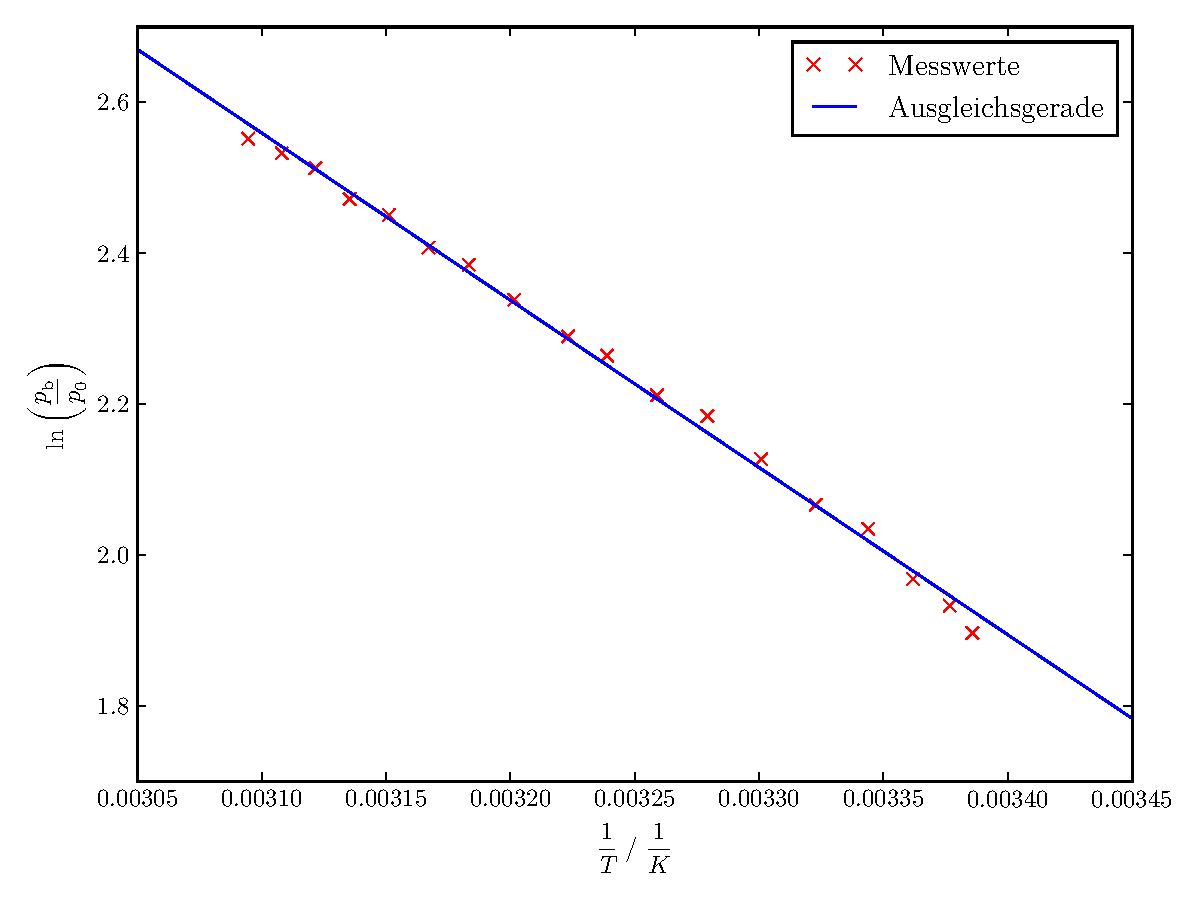
\includegraphics[width=\textwidth]{Plot2.pdf}
  \caption{Druck des Transportmediums in Abhängigkeit von der Temperatur des Wassers.}
  \label{fig:plot2}
\end{figure}

Mit den Werten für $\sfrac{\symup{d} T_2 \left( t \right)}{\symup{d} t}$ aus Tabelle \ref{tab:ergebnisse1}
und den Formeln \eqref{eqn:massendurchsatz} und \eqref{eqn:massen_umsatz} wird dann
der Massendurchsatz von $Cl_2F_2C$ berechnet. Die Ergebnisse dazu stehen in Tabelle
\ref{tab:ergebnisse2}.
\begin{table}
  \centering
  \caption{Massendurchsatz des Transportmediums in $\si{\mol\per\second}$ und in $\si{\gram\per\second}$.}
  \label{tab:ergebnisse2}
  \sisetup{table-format=3.2}
  \begin{tabular}{S S S}
    \toprule
    {$\frac{\symup{d} m}{\symup{d} t} \,/\, \si{\mol\cdot\second\tothe{-1}}$} & {$\frac{\symup{d} m}{\symup{d} t} \,/\, \si{\gram\cdot\second\tothe{-1}}$} & {$T_2 \,/\, \si{\kelvin}$}\\
    \midrule
    \num{-1.10(5)e-2} & \num{-1.3(1)e-2} & 294.15\\
    \num{-2.2(1)e-2} & \num{-2.7(1)e-2} & 286.15\\
    \num{-1.6(1)e-2} & \num{-2.0(1)e-2} & 277.55\\
    \num{-1.1(1)e-2} & \num{-1.1(1)e-2} & 273.15\\
    \bottomrule
  \end{tabular}
\end{table}
Die Fehler wurden ebenfalls mit Python bestimmt und die entsprechende Ableitung
für Formel \eqref{eqn:formelgauß} lautet:
\begin{equation}
  \frac{\partial \frac{\symup{d} m}{\symup{d} t}}{\partial \frac{\symup{d} T_2 \left( t \right)}{\symup{d} t}} = \frac{(m_2 c_{\mathup{w}}+m_{\mathup{k}}c_{\mathup{k}})}{L}.
\end{equation}\\

\subsection{Bestimmung der mechanischen Leistung}
Zuletzt wird die mechanische Leistung berechnet, die der Kompressor aufwenden muss.
Dazu werden die Formeln~\eqref{eqn:Leistung}~--~\eqref{eqn:dichte}, die Werte
für $p_\mathup{a}$ und $p_\mathup{b}$ aus Tabelle \ref{tab:messwerte2} sowie der
Massendurchsätzen verwendet.
Folgende Werte waren hierzu mit der Anleitung gegeben:
\begin{align}
  \kappa &= 1.14 & &\rho_0 \left( \SI{0}{\celsius} \right) = \SI{5.51}{\gram\per\liter} = \SI{5510}{\gram\per\meter\tothe{3}}\\
  T_0 &= \SI{273.15}{\kelvin} & &p \left( \SI{0}{\celsius} \right) = \SI{1}{\bar}
\end{align}
Als Zwischenergebnis stehen in Tabelle \ref{tab:dichten} die nach Formel \eqref{eqn:dichte}
bestimmten Dichten des Mediums zur entsprechenden Temperatur $T_2$.
\begin{table}
  \centering
  \caption{Dichte des Transportmediums mit der jeweiligen Temperatur $T_2$.}
  \label{tab:dichten}
  \sisetup{table-format=3.2}
  \begin{tabular}{S S S}
    \toprule
    {$\rho \,/\, \si{\gram\meter\tothe{-3}}$} & {$T_2 \,/\, \si{\kelvin}$}\\
    \midrule
    \num{-1.3(1)e-2} & 294.15\\
    \num{-2.7(1)e-2} & 286.15\\
    \num{-2.0(1)e-2} & 277.55\\
    \num{-1.1(1)e-2} & 273.15\\
    \bottomrule
  \end{tabular}
\end{table}\\
Mit diesen ergeben sich schließlich nach Formel \eqref{eqn:Leistung} die in
Tabelle \ref{tab:ergebnisse3} stehenden Werte für die mechanische Leistung
und den Wirkungsgrad der Apparatur.
\begin{table}
  \centering
  \caption{Mechanische Leistung des Kompressors und Wirkungsgrad bei den jeweiligen Temperaturen $T_2$.}
  \label{tab:ergebnisse3}
  \sisetup{table-format=3.2}
  \begin{tabular}{S S S}
    \toprule
    {$\left| N_\mathup{mech} \right| \,/\, \si{\watt}$} & {$\frac{\left| N_\mathup{mech} \right|}{N} \,/\, \si{\percent}$} & {$T_2 \,/\, \si{\kelvin}$}\\
    \midrule
    \num{24(1)} & \num{14(1)} & 294.15\\
    \num{49(3)} & \num{24(1)} & 286.15\\
    \num{43(3)} & \num{20(1)} & 277.55\\
    \num{32(3)} & \num{15(1)} & 273.15\\
    \bottomrule
  \end{tabular}
\end{table}\\
Die Fehler wurden erneut mit Python bestimmt und die Ableitung für Formel \eqref{eqn:formelgauß}
lautet:
\begin{equation}
  \frac{\partial N_{\mathup{mech}}}{\partial \frac{\symup{d} m}{\symup{d} t}}=\frac{1}{κ-1}\left(p_{\mathup{b}}\sqrt[κ]{\frac{p_{\mathup{a}}}{p_{\mathup{b}}}}-p_{\mathup{a}}\right)\frac{1}{ρ}.
\end{equation}
\section{Diskussion}
\label{sec:diskussion}
\begin{table}
  \centering
  \caption{Ergebnisse des Versuchs.}
  \label{tab:ergebnisse4}
  \sisetup{table-format=3.2}
  \begin{tabular}{S S S S S S}
    \toprule
    {$\left| N_\mathup{mech} \right| \,/\, \si{\watt}$} & {$\frac{\left| N_\mathup{mech} \right|}{N} \,/\, \si{\percent}$} & {$\nu$} & {$\nu_\mathup{id}$} & {$T_2 \,/\, \si{\kelvin}$} & {$T_1 \,/\, \si{\kelvin}$}\\
    \midrule
    \num{24(1)} & \num{14(1)} & \num{1.7(1)} & 148.1 & 294.15 & 296.15\\
    \num{49(3)} & \num{24(1)} & \num{2.0(2)} & 16.2 & 286.15 & 304.95\\
    \num{43(3)} & \num{20(1)} & \num{1.9(4)} & 8.6 & 277.55 & 314.15\\
    \num{32(3)} & \num{15(1)} & \num{1.4(6)} & 6.8 & 273.15 & 320.35\\
    \bottomrule
  \end{tabular}
\end{table}
In Tabelle \ref{tab:ergebnisse4} sind noch einmal die Ergebnisse des Versuchs angegeben.
Grundsätzlich ist der Versuch sehr anschaulich. Z.B. wird an ihm die Funktionsweise
von entsprechenden technischen Geräten, wie Kühlschränken, sehr verständlich dargestellt.
Die berechneten Werte der realen Güte weichen um $\SI{79.4}{\percent}$ ($T_1 = \SI{320.35}{\kelvin}$)
bis $\SI{98.9}{\percent}$ ($T_1 = \SI{296.15}{\kelvin}$) von den idealen Werten
ab, was unter anderem daran liegt, dass die Apparatur nicht optimal Isoliert
ist und es so zu einigen Energieverlusten kommt. Genauso wurde angenommen, dass
der Kompressor die Luft adiabatisch komprimiert, also ohne Wärmeabgabe
an die Umgebung, was nur bedingt der Fall ist. Der Verlust über die
Isolierung scheint allerdings größer zu sein, da bei den "Deckeln" der
Behälter, über eine größere Lücke, ein fast direkter Wärmeaustausch mit der Umgebung möglich war und die
Kompression laut \cite{anleitung} nahezu adiabatisch verläuft.\\

Bei der Recherche haben wir festgestellt, dass es unüblich ist bei Wärmepumpen
einen Wirkungsgrad anzugeben. Stattdessen wird in der Regel eine Leistungszahl
verwendet, die der in diesem Versuch bestimmten Güteziffer entspricht. Diese liegt
bei elektronischen Wärmepumpen im Normalfall zwischen 3 und 6 \cite{ibs}.
Die von uns berechneten Güten erreichen maximal einen Wert von $\num{2.0(2)}$.
\clearpage
\nocite{*}
\printbibliography

\end{document}
